%%%%%%%%%%%%%%%%%%%%%%%%%%%%%%%%%%%%%%%%%%%%%%%%%%%%%%%
% A template for Wiley article submissions.
% Developed by Overleaf.
%
% Please note that whilst this template provides a
% preview of the typeset manuscript for submission, it
% will not necessarily be the final publication layout.
%
% Usage notes:
% The "blind" option will make anonymous all author, affiliation, correspondence and funding information.
% Use "num-refs" option for numerical citation and references style.
% Use "alpha-refs" option for author-year citation and references style.

\documentclass[num-refs]{wiley-article}
% \documentclass[blind,alpha-refs]{wiley-article}

% Add additional packages here if required
\usepackage{siunitx}

% Update article type if known
% \papertype{Original Article}
% Include section in journal if known, otherwise delete
\paperfield{Journal Section}

\title{Supplementary for "Cytoskeletal and motility changes in human MSCs associated with nuclear-cytoplasmic RhoА redistribution during replicative senescence"}

% List abbreviations here, if any. Please note that it is preferred that abbreviations be defined at the first instance they appear in the text, rather than creating an abbreviations list.
% \abbrevs{ABC, a black cat; DEF, doesn't ever fret; GHI, goes home immediately.}

% Include full author names and degrees, when required by the journal.
% Use the \authfn to add symbols for additional footnotes and present addresses, if any. Usually start with 1 for notes about author contributions; then continuing with 2 etc if any author has a different present address.
\abbrevs{MSCs, mesenchymal stem cells;  PCA, principal component analisysu }

% Include full author names and degrees, when required by the journal.
% Use the \authfn to add symbols for additional footnotes and present addresses, if any. Usually start with 1 for notes about author contributions; then continuing with 2 etc if any author has a different present address.
\author[1\authfn{1}]{Danila Bobkov}
\author[2\authfn{2}]{Anastasia Polyanskaya}
\author[1\authfn{1}]{Anastasia Musorina}
\author[1\authfn{1}]{Ekaterina Lomert}
\author[1\authfn{1}]{Sergey Shabelnikov}
\author[1\authfn{1}]{Galina Poljanskaya}

% \contrib[\authfn{1}]{Equally contributing authors.}

% Include full affiliation details for all authors
\affil[1]{Institute of Cytology of the Russian Academy of Science, 194064 Tikhoretsky ave. 4, St-Petersburg, Russia }
\affil[2]{Peter the Great St. Petersburg Polytechnic University, Polytechnicheskaya, 29,  St.Petersburg, 195251, Russia}

\corraddress{Tikhoretsky ave. 4, St-Petersburg, 194064, Russia}
\corremail{bobkov@incras.ru}

\presentadd[\authfn{2}]{Peter the Great St. Petersburg Polytechnic University, Polytechnicheskaya, 29,  St.Petersburg, 195251, Russia}
\iffalse
\author[1\authfn{1}]{Author One PhD}
\author[2\authfn{1}]{Author A.~Two MD}
\author[2\authfn{2}]{Author Three PhD}
\author[2]{Author B.~Four}

\contrib[\authfn{1}]{Equally contributing authors.}

% Include full affiliation details for all authors
\affil[1]{Department, Institution, City, State or Province, Postal Code, Country}
\affil[2]{Department, Institution, City, State or Province, Postal Code, Country}

\corraddress{Author One PhD, Department, Institution, City, State or Province, Postal Code, Country}
\corremail{correspondingauthor@email.com}

\presentadd[\authfn{2}]{Department, Institution, City, State or Province, Postal Code, Country}

\fundinginfo{Funder One, Funder One Department, Grant/Award Number: 123456, 123457 and 123458; Funder Two, Funder Two Department, Grant/Award Number: 123459}
\fi
% Include the name of the author that should appear in the running header
\runningauthor{Bobkov et al. Motility changes in aging MSCs}

\begin{document}

\maketitle

\iffalse
\begin{abstract}
This is a generic template designed for use by multiple journals, which includes several options for customization. Please consult the author guidelines for the journal to which you are submitting in order to confirm that your manuscript will comply with the journal's requirements. Please replace this text with your abstract.

% Please include a maximum of seven keywords
\keywords{keyword 1, \emph{keyword 2}, keyword 3, keyword 4, keyword 5, keyword 6, keyword 7}
\end{abstract}


\section{First Level Heading}

Please lay out your article using the section headings and example objects below, and remember to delete all help text prior to submitting your article to the journal.

\begin{figure}[bt]
\centering

\includegraphics[width=6cm]{example-image-rectangle}
\caption{Although we encourage authors to send us the highest-quality figures possible, for peer-review purposes we are can accept a wide variety of formats, sizes, and resolutions. Legends should be concise but comprehensive – the figure and its legend must be understandable without reference to the text. Include definitions of any symbols used and define/explain all abbreviations and units of measurement.}
\end{figure}

\subsection{Second Level Heading}
If data, scripts or other artefacts used to generate the analyses presented in the article are available via a publicly available data repository, please include a reference to the location of the material within the article.

% Equations should be inserted using standard LaTeX equation and eqnarray environments, not as graphics, and should be set in the main text
This is an equation, numbered
\begin{equation}
\int_0^{+\infty}e^{-x^2}dx=\frac{\sqrt{\pi}}{2}
\end{equation}
And one that is not numbered
\begin{equation*}
e^{i\pi}=-1
\end{equation*}

\subsection{Adding Citations and a References List}

Please use a \verb|.bib| file to store your references. When using Overleaf to prepare your manuscript, you can upload a \verb|.bib| file or import your Mendeley, CiteULike or Zotero library directly as a \verb|.bib| file\footnote{see \url{https://www.overleaf.com/blog/184}}. You can then cite entries from it, like this: \cite{lees2010theoretical}. Just remember to specify a bibliography style, as well as the filename of the \verb|.bib|.

You can find a video tutorial here to learn more about BibTeX: \url{https://www.overleaf.com/help/97-how-to-include-a-bibliography-using-bibtex}.

This template provides two options for the citation and reference list style:
\begin{description}
\item[Numerical style] Use \verb|\documentclass[...,num-refs]{wiley-article}|
\item[Author-year style] Use \verb|\documentclass[...,alpha-refs]{wiley-article}|
\end{description}

\subsubsection{Third Level Heading}
Supporting information will be included with the published article. For submission any supporting information should be supplied as separate files but referred to in the text.

Appendices will be published after the references. For submission they should be supplied as separate files but referred to in the text.

\paragraph{Fourth Level Heading}
% Here are examples of quotes and epigraphs.
\begin{quote}
The significant problems we have cannot be solved at the same level of thinking with which we created them.\endnote{Albert Einstein said this.}
\end{quote}

\begin{epigraph}{Albert Einstein}
Anyone who has never made a mistake has never tried anything new.
\end{epigraph}

\subparagraph{Fifth level heading}
Measurements should be given in SI or SI-derived units.
Chemical substances should be referred to by the generic name only. Trade names should not be used. Drugs should be referred to by their generic names. If proprietary drugs have been used in the study, refer to these by their generic name, mentioning the proprietary name, and the name and location of the manufacturer, in parentheses.

\begin{table}
\caption{This is a table. Tables should be self-contained and complement, but not duplicate, information contained in the text. They should be not be provided as images. Legends should be concise but comprehensive – the table, legend and footnotes must be understandable without reference to the text. All abbreviations must be defined in footnotes.}
\begin{threeparttable}
\begin{tabular}{lccrr}
\headrow
\thead{Variables} & \thead{JKL ($\boldsymbol{n=30}$)} & \thead{Control ($\boldsymbol{n=40}$)} & \thead{MN} & \thead{$\boldsymbol t$ (68)}\\
Age at testing & 38 & 58 & 504.48 & 58 ms\\
Age at testing & 38 & 58 & 504.48 & 58 ms\\
Age at testing & 38 & 58 & 504.48 & 58 ms\\
Age at testing & 38 & 58 & 504.48 & 58 ms\\
\hiderowcolors
stop alternating row colors from here onwards\\
Age at testing & 38 & 58 & 504.48 & 58 ms\\
Age at testing & 38 & 58 & 504.48 & 58 ms\\
\hline  % Please only put a hline at the end of the table
\end{tabular}

\begin{tablenotes}
\item JKL, just keep laughing; MN, merry noise.
\end{tablenotes}
\end{threeparttable}
\end{table}

\fi

\section{Tables}

\begin{table}[hbt!]
  \caption{Cheddock scale for Kendall correlation coefficient estimation}
  \label{cheddock}
\centering
\begin{tabular}{l|c|}
  Tau-Kendall Correlation coeff value & Colocalization \\
 \hline
 $ <0.1 $ & no link \\
 0.1-0.3 & weak \\
 0.3-0.5 & moderate \\
 0.5-0.7 & noticeable \\
 0.7-0.9 & high \\
 0.9-0.99 & very high
\end{tabular}
\end{table}

% latex table generated in R 3.6.1 by xtable 1.8-4 package
\begin{table}[hbt!]
  \label{tab:pca-M9}
  \caption{PCA of myosin-9/F-actin colocalization data loadings for 2 factors}
\centering
\begin{tabular}{c|rrrrr}
  \hline
  & Rval & tM1 & tM2 & bTau & Rs \\
  \hline
Factor 1 & 0.77 & 0.91 & 0.97 & 0.19 & 0.23 \\
  Factor 2 & 0.46 & 0.13 & 0.17 & 0.98 & 0.96 \\
Uniqueness &  0.198 & 0.159 & 0.039 & 0.005 & 0.024 \\
   \hline
\end{tabular}
\end{table}

\begin{table}[hbt!]
  \caption{Kruskal-Wallis rank sum test results for myosin-9/F-actin colocalization coefficients}
  \label{tab:M9colocs}
\centering
\begin{tabular}{l|ccc}
    \hline
 Colocalization coefficient & chi-squared & df & p-value  \\
   \hline
 Kendall's Tau-b & 34.669 & 10 & 0.0001422 \\
 Spearman's R & 34.373 & 10 &  0.0001596 \\
 Manders' M & 16.107 & 10 & 0.09661 \\
 Pearson's R & 15.152 & 10 & 0.1266
\end{tabular}
\end{table}

\begin{table}[hbt!]
  \caption{Logistic regression with myosin-9/F-actin colocalization coefficients as predictors and passage numger as fitted values}
  \label{glm-M9-Fact}
\centering
\begin{tabular}{lrrrrr}
  \hline
 & Df & Deviance & Resid. Df & Resid. Dev & Pr($>$Chi) \\
  \hline
NULL &  &  & 115 & 68.13 &  \\
  Rval & 1 & 0.95 & 114 & 67.18 & 0.3295 \\
  tM1 & 1 & 0.91 & 113 & 66.27 & 0.3407 \\
  tM2 & 1 & 1.32 & 112 & 64.96 & 0.2510 \\
  bTau & 1 & 4.14 & 111 & 60.82 & 0.0419 * \\
  Rs & 1 & 0.20 & 110 & 60.61 & 0.6509 \\
   \hline
\end{tabular}
\end{table}

\begin{table}[hbt!]
  \caption{Logistic regression with $\alpha$-actinin-4 and nucleus colocalization coefficients as predictors and passage numbers as fitted values}
  \label{glm-aA4-nuc}
\centering
\begin{tabular}{rrrrr}
  \hline
 & Estimate & Std. Error & z value & Pr($>$$|$z$|$) \\
  \hline
(Intercept) & 3.7063 & 1.6058 & 2.31 & 0.0210 \\
  bTau & 58.8841 & 22.4644 & 2.62 & 0.0088 \\
  tM1 & -0.9898 & 1.5118 & -0.65 & 0.5126 \\
  tM2 & -1.9521 & 1.6107 & -1.21 & 0.2256 \\
  Rval & -4.3852 & 1.9107 & -2.30 & 0.0217 \\
  Rs & -50.4674 & 17.4231 & -2.90 & 0.0038 \\
   \hline
\end{tabular}
\end{table}

\begin{table}[hbt!]
  \caption{Logistic regression with RhoA and nucleus colocalization coefficients as predictors and passage numger as fitted values}
  \label{glm-RhoA-nuc}
\centering
\begin{tabular}{l|rrrr}
  \hline
 & Estimate & Std. Error & z value & Pr($>$$|$z$|$) \\
  \hline
(Intercept) (**) & 2.2687 & 0.7100 & 3.20 & 0.0014 \\
  bTau (***) & 97.1021 & 27.8353 & 3.49 & 0.0005 \\
  Rval & 0.5242 & 1.3355 & 0.39 & 0.6947 \\
  Rs (***) & -78.1599 & 22.1536 & -3.53 & 0.0004 \\
   \hline
\end{tabular}
\end{table}

\begin{table}[hbt!]
  \caption{Superose 6 column Gel-filtration calibration protein set}
  \label{calibration}
\centering
\begin{tabular}{l|c|}
 Protein & Molecular weight (Mr), kDa  \\
 \hline
 Ovalbumin & 43 \\
 Horse spleen Thyroglobulin & 669 \\
 Rabbit muscle Ferritin & 440 \\
 Chicken egg white Aldolase & 158 \\
 Bovine erythrocytes Ovalbumin & 43 \\
 Bovine lung Ribonuclease A & 13.7
\end{tabular}
\begin{tablenotes}
\item
\end{tablenotes}
\end{table}

\section{Figures}

\begin{figure}[hbt!]
  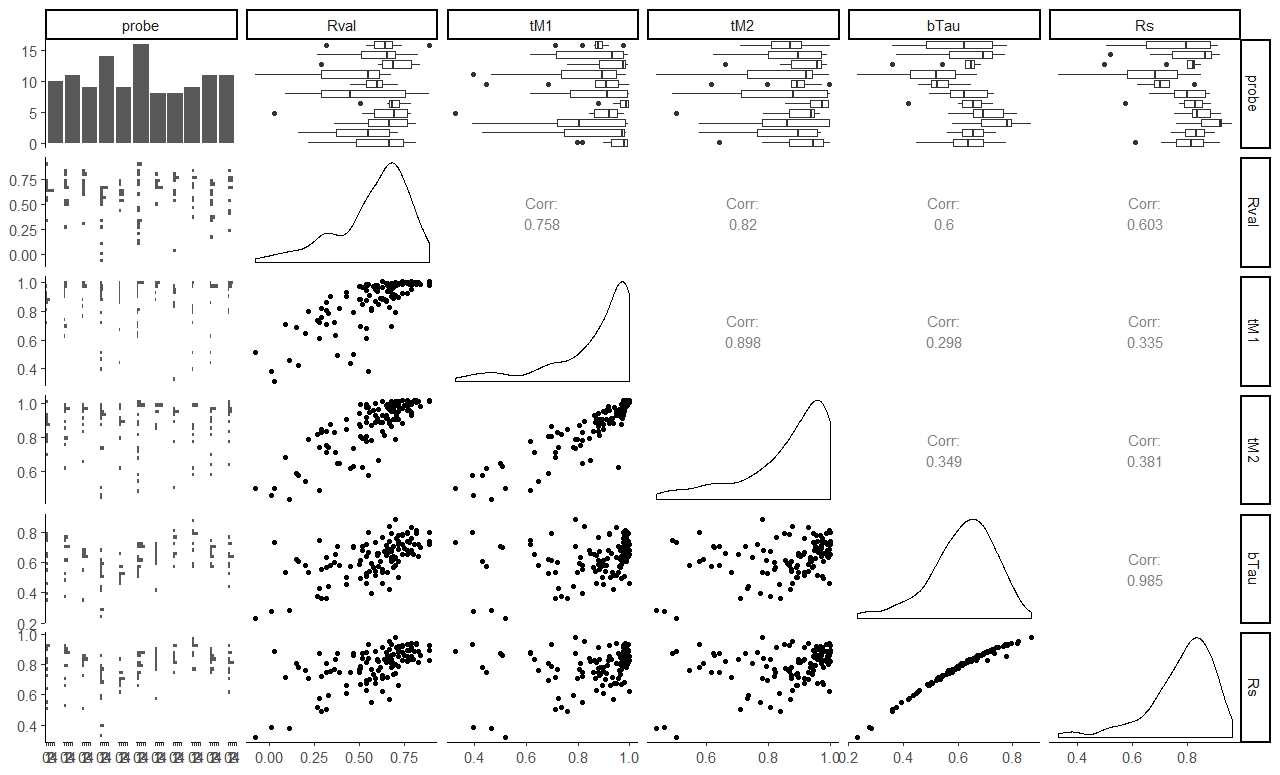
\includegraphics[width=1\linewidth]{supp1.jpeg}
  \caption{Correlation matrix of colocalization coefficients calculated in Coloc2 ImageJ plugin: Rs, Rval, tM1, tM2, bTau. Data collected in two channels from manually selected cells as ROIs in confocal images. MSCWJ-1 cells were stained with polyclonal anti-myosin-9 antibodies and rhodamine phalloidin. Cells were fixed at passages: 7, 9, 12, 15, 18, 21, 25, 27, 28, 35, 36.}
  \centering
\end{figure}

\begin{figure}[hbt!]
  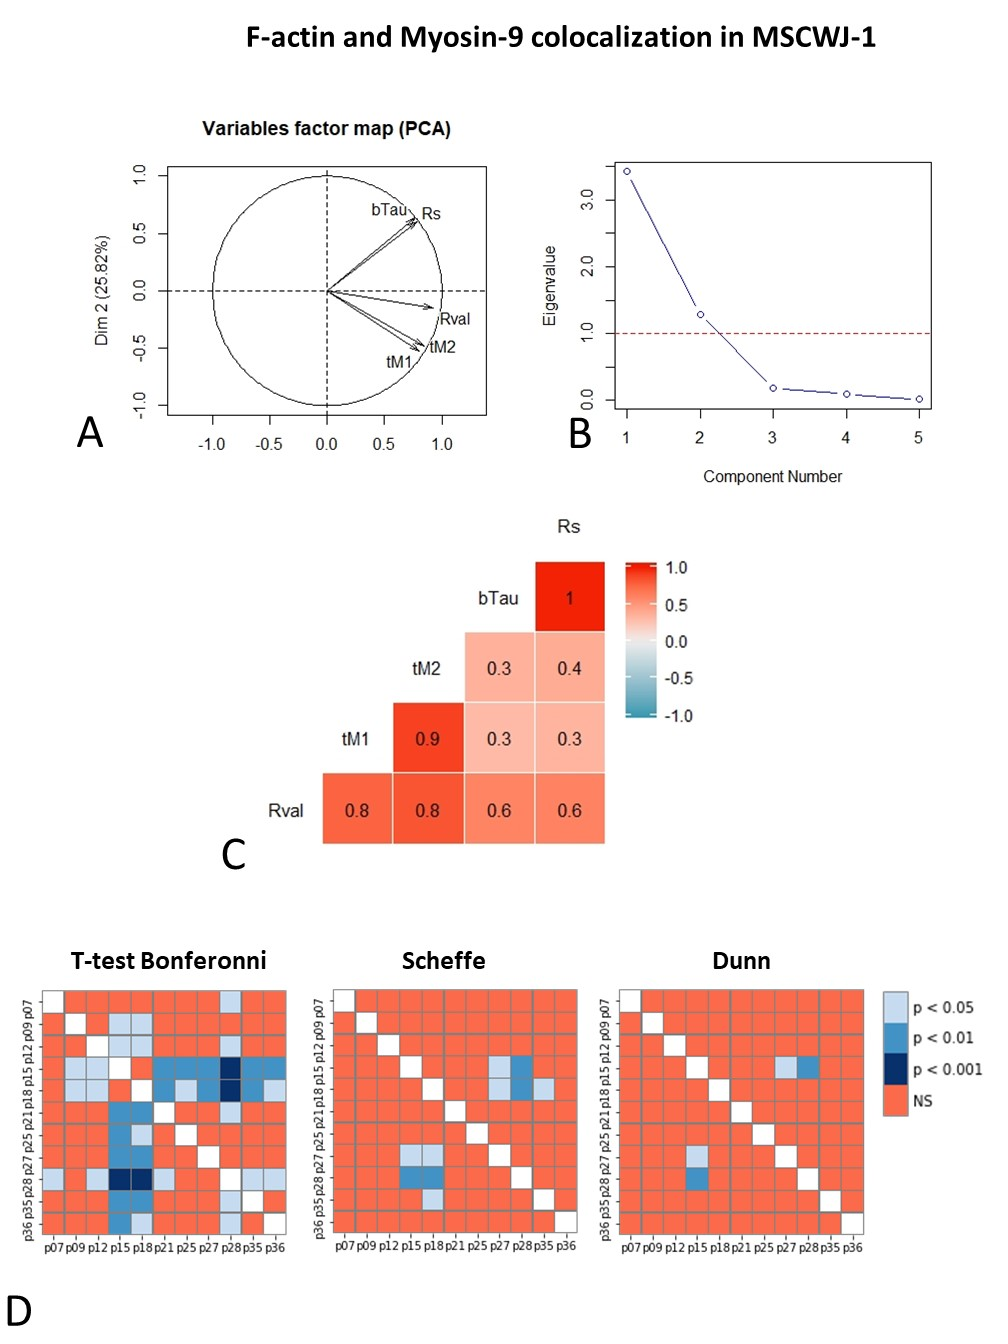
\includegraphics[width=1\linewidth]{supp2.jpg}
  \caption{Explorative analisys of colocalization data.
  PCA factor map (A) and scree plot (B) for colocolization coefficients. Correlation plots for myosin-9/F-actin (C) and alpha-actinin-4/F-actin colocalization coefficients. (E) Pairwise comparison post hoc tests for myosin-9/F-actin bTau coefficient. Data collected in two channels from manually selected cells as ROIs in confocal images. MSCWJ-1 cells were stained with polyclonal anti-myosin-9 antibodies and rhodamine phalloidin. Cells were fixed at passages: 7, 9, 12, 15, 18, 21, 25, 27, 28, 35, 36.}
  \centering
\end{figure}


\printendnotes

% Submissions are not required to reflect the precise reference formatting of the journal (use of italics, bold etc.), however it is important that all key elements of each reference are included.
% \bibliography{sample}
\iffalse
\begin{biography}[example-image-1x1]{A.~One}
Please check with the journal's author guidelines whether author biographies are required. They are usually only included for review-type articles, and typically require photos and brief biographies (up to 75 words) for each author.
\bigskip
\bigskip
\end{biography}

\graphicalabstract{example-image-1x1}{Please check the journal's author guildines for whether a graphical abstract, key points, new findings, or other items are required for display in the Table of Contents.}

Recommended
Alexis Gautreau
alexis.gautreau@lebs.cnrs-gif.fr
École Polytechnique
Laboratoire d'Enzymologie et Biochimie

Recommended
Roman Gorelik
roman.gorelik@lebs.cnrs-gif.fr
Ecole Polytechnique
Laboratoire d'Enzymologie et Biochimie

Recommended
Tatyana Svitkina
svitkina@sas.upenn.edu
University of Pennsylvania

Recommended
Antonina Alexandrova
tonya_alex@yahoo.com
FBGU National Medical Research Center of Oncology named after N N Blokhin Research Institute of Carcinogenesis
\fi
\end{document}
